\documentclass[a4paper]{article}
\usepackage{amsfonts}
\usepackage{amsmath}
\usepackage{amssymb}
\usepackage{graphicx}
\usepackage{float}     

\begin{document}
  
\noindent \large Auteur: Siebe Mees \\
\noindent \large Studierichting: Informatica\\
\noindent \large Oefeningenreeks 3G nr. 13.2\\

\medskip

\normalsize

$f(x)=\sin 3x$\\

\begin{enumerate}

\item Domein\\

$Dom\ f=\mathbb{R}$\\

$p = \sin 3x \Leftrightarrow 3x = 2\pi \Leftrightarrow x = \dfrac{2\pi}{3}$\\

$\Rightarrow $ Beperkte periode $:\left[0,\dfrac{2\pi}{3}\right]$\\


\item Asymptoten\\

er zijn geen asymptoten.\\


\item Tekenonderzoek van $f(x)$\\

$\sin 3x=0$\\

$3x=k\pi $\\

$x=\dfrac{k\pi}{3}$\\

$\Rightarrow f^{(-1)}(0)=\left\{0,\dfrac{\pi}{3},\dfrac{2\pi}{3}\right\}$\\

\begin{tabular}{c|ccccc}
$x$ & $0$ &  & $\dfrac{\pi}{3}$ &  & $\dfrac{2\pi}{3}$ \\ \hline
$f(x)$ & $0$ & $+$ & $0$ & $-$ & $0$
\end{tabular}\\


\item Tekenonderzoek van $f'(x)$\\

$f(x)=\sin 3x$\\

$f'(x)=3\cos 3x$\\

$3\cos 3x=0$\\

$\cos 3x=0$\\

$3x=\dfrac{\pi}{2}+k\pi $\\

$x=\dfrac{\pi}{6}+\dfrac{k\pi}{3} $\\

$\Rightarrow f'^{(-1)}(0)=\left\{\dfrac{\pi}{6},\dfrac{\pi}{2}\right\}$\\

\begin{tabular}{c|ccccc}
$x$ & $0$ & $\dfrac{\pi}{6}$ &  & $\dfrac{\pi}{2}$ & \\ \hline
$f'(x)$ & $+$ & $0$ & $-$ & $0$ & $+$
\end{tabular}\\

$M\left(\dfrac{\pi}{6}\right)=\sin \left(3\cdot\dfrac{\pi}{6}\right)$\\

$M\left(\dfrac{\pi}{6}\right)=1$\\

$\Rightarrow M\left(\dfrac{\pi}{6},1\right)$\\

$m\left(\dfrac{\pi}{2}\right)=\sin \left(3\cdot\dfrac{\pi}{2}\right)$\\

$m\left(\dfrac{\pi}{2}\right)=-1$\\

$\Rightarrow m\left(\dfrac{\pi}{2},-1\right)$\\


\item Tekenonderzoek van $f''(x)$\\

$f'(x)=3\cos 3x$\\

$f''(x)=-9\sin 3x$\\

$-9\sin 3x=0$\\

$\sin 3x=0$\\

$3x=k\pi$\\

$x=\dfrac{k\pi}{3}$\\

$\Rightarrow f''^{(-1)}(0)=\left\{0,\dfrac{\pi}{3},\dfrac{2\pi}{3}\right\}$\\

\begin{tabular}{c|ccccc}
$x$ & $0$ &  & $\dfrac{\pi}{3}$ &  & $\dfrac{2\pi}{3}$ \\ \hline
$f''(x)$ & $0$ & $-$ & $0$ & $+$ & $0$
\end{tabular}\\

$B\left(\dfrac{\pi}{3}\right)=\sin \left(3\cdot\dfrac{\pi}{3}\right)$\\

$B\left(\dfrac{\pi}{3}\right)=0$\\

$\Rightarrow B\left(\dfrac{\pi}{3},0\right)$\\

\item Schets\\

\begin{figure}[H]
\centering
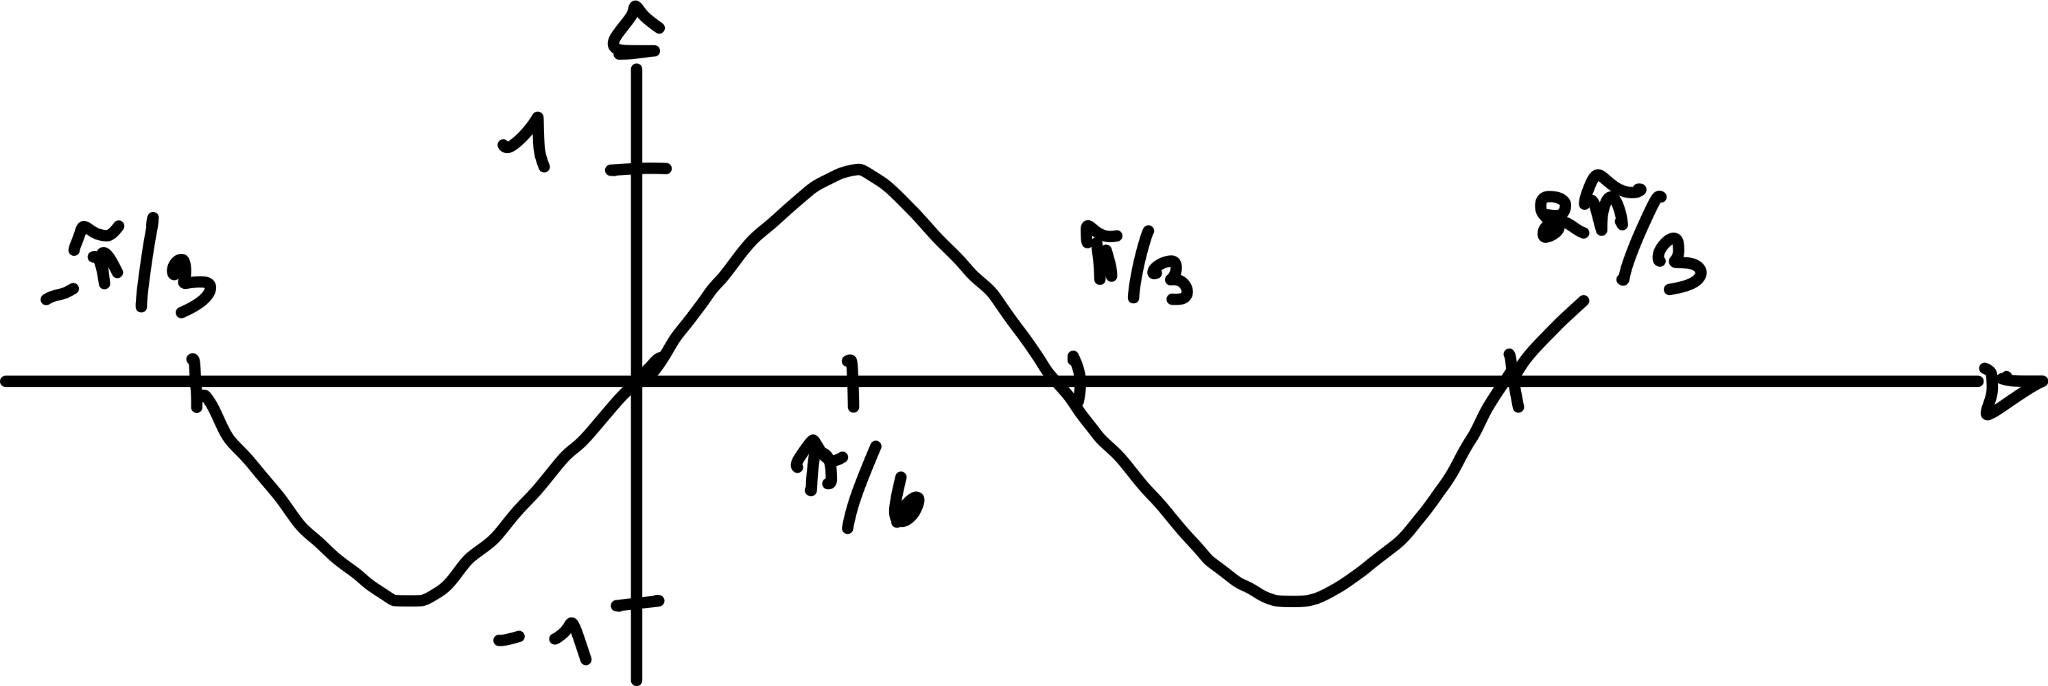
\includegraphics[width=5cm]{3G-13.2-siebe.mees.INF.png}
\end{figure}

\end{enumerate}

$\Rightarrow$ Samenvattende tabel\\

\begin{tabular}{c|ccccc}
$x$ & $0$ & $\dfrac{\pi}{6}$ & $\dfrac{\pi}{3}$ & $\dfrac{\pi}{2}$ & $\dfrac{2\pi}{3}$ \\ \hline
$f(x)$ & $0$ & $+$ & $0$ & $-$ & $0$ \\
$f'(x)$ & $+$ & $0$ & $-$ & $0$ & $+$ \\
$f''(x)$ & $0$ & $+$ & $0$ & $-$ & $0$ \\ \hline
$f(x)$ & $\nearrow$ & $M(1)$ & $\searrow$ & $m(-1)$ & $\nearrow$ \\
 &  & $\smile$ & $B(0)$ & $\frown$ &
\end{tabular}\\

\begin{thebibliography}{999}
%\bibitem{a} Referentie
\end{thebibliography}
\end{document} 
